\documentclass[10pt]{article}%

\usepackage{algpseudocode, algorithm2e}
\usepackage{polski}
\usepackage[utf8]{inputenc}
\usepackage{flexisym}
\usepackage{graphicx}
\usepackage{caption}
\usepackage{float}



\begin{document}

\section*{AiSD wszystkie - wersja z dnia \today}




\subsection*{Drzewa AVL}
\begin{enumerate}
\item (Zad. 12, 06.2017) Jak mocno można ograniczyć (w pesymistycznym przypadku) liczbę rotacji podczas usuwania wierzchołka z drzewa AVL o $n$ wierzchołkach? Uzasadnij, że nie da się bardziej niż podałeś(aś).

\item (Zad. 19, 06.2016) Jaką największą wysokość może mieć drzewo AVL zawierające 67 kluczy? Odpowiedź uzasadnij.

\item (Zad. 14, 06.2015) Jeśli w drzewach AVL zmienilibyśmy warunek, by poddrzewa mogły różnić się o 2 (nie o 1) wysokością, to Czy drzewo n-wierzchołkowe dalej ma wysokość $\Theta(n)$? 

\end{enumerate}
\subsection*{Reszta do zrobienia}
\begin{enumerate}

\item(Zad. 1, 06.2017)
Opisz algorytm oparty na programowaniu dynamicznym wyznaczający optymalną kolejność mnożenia macierzy. Jaka jest jego złożoność? Jeśli jest to algorytm podany na wykładzie, możesz na tym poprzestać, w przeciwnym razie uzasadnij jego poprawność i złożoność.


\item (Zad. 2, 06.2017) Ile maksymalnie operacji \textit{join} wykona się podczas łączenia kopców dwumianowych (wersja eager), z których każdy zawiera nie więcej niż 500 elementów? Przypomnienie: operacja \textit{join} łączy dwa drzewa dwumianowe tego samego rzędu.
\item (Zad. 3, 06.2017) Narysuj 
\begin{itemize}
\item drzewo \emph{Splay} po wykonaniu na początkowo pustym drzewie ciągu operacji:
 $$insert(n),insert(n-1),insert(n-2),...,(insert(1),$$
 \item drzewo \emph{Splay} po wykonaniu operacji \emph{Splay(n), Splay(n-1)} na drzewie otrzymanym w poprzednim punkcie
 \end{itemize}

\item(Zad. 4, 06.2017) Podaj przykład drzewca (tj. podaj wartość kluczy wraz z przydzielonymi im priorytetami) o n wierzchołkach, w którym każdy wierzchołek wewnętrzny ma tylko prawego syna. Następnie podaj, który wierzchołek będzie wymagał najwięcej rotacji podczas ustawiania go. Ile to będzie rotacji? Odpowiedź uzasadnij.

\item (Zad. 5, 06.2017) Dolną granicę $\lceil \frac{3}{2} n - 2 \rceil $ na liczbę porównań niezbędnych do wyznaczenia \emph{max} i \emph{min} w zbiorze \emph{n} elementów można wykazać stosując grę z adwersarzem. Opisz skuteczną strategię w takiej grze. Jeśli jest to strategia opisana na wykładzie, możesz na tym poprzestać. Jeśli jest to inna strategia, wykaż, że jest skuteczna.

\item (Zad. 6, 06.2017) Rozważamy haszowanie metodą adresowania otwartego, w której konflikty rozwiązujemy metodą liniową. Pokaż, że po umieszczeniu $n/2$ kluczy w tablicy $n$ elementowej, mogą istnieć dwie lokalizacje w tej tablicy, do których kolejny (tj. ($n/2 + 1$)szy) klucz ma szansę trafić z prawdopodobieństwem $1/n$.

\item (Zad. 7, 06.2017) Opisz w jaki sposób wybierany jest \emph{pivot} w każdym z następujących z następujących algorytmów znajdowania $k$-tego elementu: 
\begin{itemize}
\item Algorytm Hoare'a,
\item Algorytm Magicznych Piątek,
\item Lazy Select.
\end{itemize}

\item (Zad. 8, 06.2017) Czy istnieje wzorzec o długości $n$ (dla dowolnego $n>5$) nad alfabetem $\{a,b\}$, dla którego maksymalna wartość funkcji prefiksowej $\pi$ jest równa 
\begin{itemize}
\item[a] 0,
\item[b] 1?
\end{itemize}
 
\item (Zad. 09, 06.2017) Rozważamy \emph{B} drzewa, których wierzchołki mogą pamiętać od dwóch do czterech kluczy. Narysuj, jak będzie wyglądać takie \emph{B} drzewo po wstawieniu do początkowego pustego drzewa kolejno klucz $1,2,\ldots,10$.

\item (Zad. 10, 06.2017) Porównaj trudność problemu sprowadzania izomorfizmu drzew ukorzenionych i problemu sprawdzaniaa izomorfizmu drzew nieukorzenionych.

\item (Zad. 11, 06.2017) W algorytmie \emph{Shift And} wykorzystywane są operacje logiczne na słowach maszynowych. Wytłumacz, w jaki sposób?

\item (Zad. 13, 06.2017) Niech $T_{1}$ oznacza najmniejsze pod względem liczby wierzchołków drzewo o rzędzie $i$, które może zawierać kopiec Fibonacciego. Narysuj drzewa $T_{i}$, dla $i = 0,1,\ldots,6$.

\item (Zad. 14, 06.2017)W jaki sposób, stosując iloczyn wektorowy można sprawdzić, czy dwa punkty (powiedzmy $p_1$ i $p_2$) leżą po tej samej stronie prostej przechodzącej przez dwa punkty (powiedzmy A i B)?

\item (Zad. 15, 06.2017) Ile pamięci zajmuje słownik statyczny (oparty o haszowanie dwupoziomowe) zawierający $n$ kluczy? Co musimy w nim pamiętać oprócz samych kluczy?

\item (Zad. 16, 06.2017) Podaj definicję i przykład uniwersalnej rodziny funkcji haszujących.

\item (Zad. 17, 06.2017) Algorytm FFT używaliśmy do zamiany reprezentacji wielomianu w reprezentację jako zbiór wartości wielomianu. Uzasadnij, dlaczego FFT możemy także zastosować do zamiany odwrotnej.

\item (Zad. 18, 06.2017) W analizie problemu \emph{Union Find} wykorzystywaliśmy pojęcie rzędu wierzchołka oraz grupy rzędu. Przypomnij definicję tych pojęć. Ile maksymalnie bitów potrzebujemy przeznaczyć na pamiętanie rzędu w każdym wierzchołku?

\item (Zad. 19, 06.2017) Wyjaśnij po co oamiętane są wartości \emph{min} i \emph{max} w ja zdeh strukturze rekurencyjnej w drzewach (kolejkach van Emde Boasa)

\item (Zad. 20, 06.2017) Przypomnij sobie algorytm oparty na zasadzie \emph{Dziel i zwyciężaj}, dla problemu znajdowania najbliższej pary punktów na płaszczyźnie. Opisz trzecią fazę algorytmu, a więc tę, która następuje po wywołaniach rekurencyjnych. Jaka jest jej złożoność?

\item (Zad. 1, 06.2016) W jakim czasie można wykonać operację succ(x) w:
\begin{itemize}
\item kopcu,
\item kopcu dwumianowym,
\item kopcu Fibonacciego,
\end{itemize}
która znajduje następnik klucza znajdującego się w wierzchołku o adresie x? Przez następnik klucza $k$ rozumiemy najmniejszy występujący w kopcu klucz $k\textprime$ taki, że $k\textprime$ taki, że $ k\textprime > k$. Jeśli$k$ jest największym kluczem w kopcu, to $k\textprime = \infty$. Możesz założyć, że wszystkie klucze w kopc są unikalne. Odpowiedź uzasadnij.
\item (Zad. 2, 06.2016) Rozwiąż rozwiązanie rekurencyjne (z redukcją do pierwiastka):
$$T(n) = \left\{\begin{array}{rcl}
1&:&n=1\\
T(\sqrt{n}+O(1)&:&wpp\\
\end{array} \right.$$
Możesz ograniczyć się do rozwiązania dla $n$ mających odpowiednią postać (taką, by w trakcie redukcji argumenty dla $T$ były liczbami naturalnymi).
\item (Zad. 3, 06.2016) Narysuj sieć Benesa-Waksmana dla n = 8.
\item (Zad. 4, 06.2016) Narysuj ciąg rotacji, które zostaną wykonane w trakcie wykonywania \textbf{delete(p)} na poniższym drzewcu. Litery w wierzchołkach drzewca oznaczają klucze, a liczby w nawiasach - priorytety. Rotacje wypisz w kolejności wykonywania.
\begin{figure}[H]
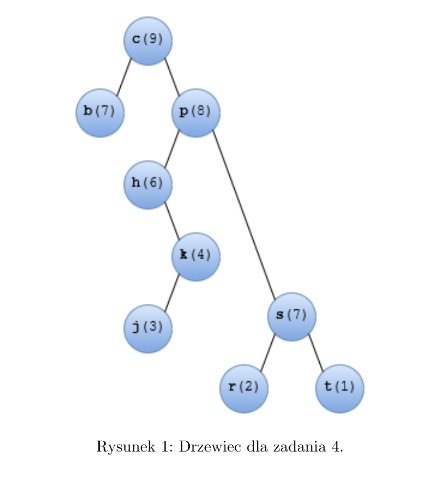
\includegraphics[scale=0.8]{z40616.png}
\caption{rys do zad 4}
\end{figure} 
\item (Zad. 5, 06.2016) Opisz ideę algorytmu klasy NC dla problemu dodawania liczb naturalnych.
\item (Zad. 6, 06.2016) Czy trójelementowe drzewo złożone z korzenia i dwóch jego synów może być drzewem splay? Odpowiedź uzasadnij.
\item (Zad. 7, 06.2016) Opisz ideę algorytmu znajdowania mediany opartego na idei próbkowania losowego.
\item (Zad. 8, 06.2016) Dlaczego algorytm \textit{Shift-And} stosowany jest jedynie do wyszukiwania krótkich wzorców?
\item (Zad. 9, 06.2016) Opisz (albo zapisz w pseudokodzie), w jaki sposób wykonywana jest operacja wstawiania klucza w drzewie van Emde Boasa.
\item (Zad. 10, 06.2016) Jaka jest największa wartość funkcji $\pi$ dla wzorca $ P = (ab)^k$? Odpowiedź uzasadnij.
\item (Zad. 11, 06.2016) W jakim czasie działa algorytm Kruskala, jeśli:
\begin{itemize}
\item krawędzie podane są w kolejności rosnących wag,,
\item kolejka priorytetowa zaimplementowana jest przy pomocy kopca Fibonacciego.
\end{itemize}
Odpowiedź uzasadnij. \textit{Uwaga: Oba te warunki są spełnione jednocześnie}
\item (Zad. 12, 06.2016) Zapisz w pseudokodzie algorytm wielomianowy, znajdujący minimalny koszt obliczenia iloczynu ciągu macierzy.
\item (Zad. 13, 06.2016) Przedstaw ideę szybkiego algorytmu sprawdzania izomorfizmu drzew. W jakim czasie działa ten algorytm?
\item (Zad. 14, 06.2016) W jakim czasie można wykonać ciąg $n$ operacji \textbf{union} i \textbf{find}, w którym wszystkie operacje \textbf{union} poprzedzają operację \textbf{find}? Odpowiedź uzasadnij 
\item (Zad. 15, 06.2016) Podaj definicję problemu plecakowego z powtórzeniami i przedstaw pseudowielomianowy algorytm rozwiązujący ten problem. Uzasadnij, że jest on pseudowielomianowy.
\item (Zad. 16, 06.2016) Jak wiadomo FFT jest algorytmem opartym na strategii Dziel i Zwyciężaj. Przedstaw redukcję wykonaną w tym algorytmie.
\item (Zad. 17, 06.2016) Napisz w pseudokodzie szybką procedurę budowy kopca. W jakim czasie działa ta procedura?
\item (Zad. 18, 06.2016) Wyjaśnij, na czym polega operacja kaskadowego odcinania w kopcu Fibonacciego.

\item (Zad. 20, 06.2016) Jaka jest oczekiwana liczba kolizji podczas wstawiania $n$ kluczy do tablicy o $ m = n^2 $ elementach, jeśli do wyznaczania miejsc wstawiania użyjemy funkcji o postaci $h(k) = ((ak + b)$ mod $p)$ mod $m$, gdzie:
\begin{itemize}
\item $p$ jest liczbą pierwszą większą od każdego ze wstawianych kluczy i większą od $m$,
\item $a$ jest losowo wybraną (z rozkładem jednostajnym liczbą z przedziału $(0, p-1]$,
\item $b$ jest losowo wybraną (z rozkładem jednostajnym liczbą z przedziału $(0, p-1]$.
\end{itemize} 
Odpowiedź uzasadnij.

\item (Zad. 1, 06.2015) Podaj przykład tekstu i wzorca dla których tablica C[0] = C[1] = C[9] = prawda, a dla pozostałych fałsz. Algorytm Shift-And.
\item (Zad. 2, 06.2015) Jak w KMR numeruje się słowa o długości 16?
\item (Zad. 3, 06.2015) Przedstaw graficznie sieć komparatorów o głębokości <= 4 sortującej wszystkie ciągi 0-1 o długości 7.
\item (Zad. 4, 06.2015) Uzasadnij, że obliczenie funkcji pi(Wzorzec[1..m]) w algorytmie KMP ma złożoność O(m).
\item (Zad. 5, 06.2015) Przedstaw macierze dla transformacji Fouriera (???) 
\item (Zad. 6, 06.2015) Podaj definicje: rząd wierzchołka i grupa rzędu wierzchołka
\item (Zad. 7, 06.2015) Czy drzewa A i B będą miały równą wysokość, jeśli przeprowadzi się na nich n operacji insert o wartościach:
\begin{itemize}
\item dla A: 1, 2, 3, ..., n 
\item dla B: n, n-1, ..., 2, 1 
\end{itemize}
\item (Zad. 8, 06.2015) Przedstaw drzewiec o n wierzchołkach, w którym usunięcie korzenia wymaga $\Omega(\sqrt{n})$ operacji, ew. podaj uzasadnienie dlaczego nie ma takiego drzewca.
\item (Zad. 9, 06.2015) Podaj rekurencyjny wzór na T(n) tak, by jego rozwiązanie było $O(\log \log n)$.
\item (Zad. 10, 06.2015) Ile jest maksymalnie drzew w kopcu:
\begin{itemize}
\item dwumianowym,
\item Fibonnaciego.
\end{itemize}
\item (Zad. 11, 06.2015) Złożoność procedury budującej kopiec (wersja z przesun-do-gory()). 
\item (Zad. 12, 06.2015) Oszacuj prawdopodobieństwo, że nie będzie żadnej kolizji podczas haszowania funkcją z uniwersalnej rodziny $\sqrt{n}$ kluczy w tablicy rozmiaru n. 
\item (Zad. 13, 06.2015) Podaj pseudowielomianowy algorytm, który wypisuje dzielniki pierwsze liczby n.

\item (Zad. 15, 06.2015) Podaj pseudokod rozwiązania problemu LCS.
\item (Zad. 16, 06.2015) Przerób kod QuickSorta na QuickSelect (selekcja k-tego elementu zamiast sortowania). Jaką ma złożoność?
\item (Zad. 17, 06.2015) Porównanie kosztów operacji { min, delmin, insert, meld } dla kopców dwumianowych w wersji Lazy i Eager.
\item (Zad. 18, 06.2015) 
\begin{itemize}
\item Podaj definicje rzędu drzewa w kopcu Fibbonaciego, 
\item Podaj górne ograniczenie na ten rząd, 
\item Podaj ideę dowodu tego ograniczenia. 
\end{itemize}
\item (Zad. 19, 06.2015) Podaj wzór rekurencyjny algorytmu magicznych piątek dla podziału na 7 elementów. 
\item (Zad. 20, 06.2015) Przykład grafu pełnego o n wierzchołkach takiego, że algorytm Boruvki znajdzie MST w jednej fazie.
\end{enumerate}

\end{document}
